\subsubsection{Completeness} \label{odp_completeness}
% Subsection structure:
% Problem: what is the generalized problem?
% 	Motivation: why is this problem scientifically important and/or interesting?
% Solution: conceptual description of solution, including formal definition of GODP and SHACL shapes.
% 	Illustration: images of GODP structure.
% 	(Statistical)Analysis: how does the solution solve the problem?
% 	Evaluation: are the results significant? What is the impact?
\paragraph{Detecting completeness}
A decision-maker makes a decision knowing context-relevant information for that specific decision. Some information crucial for decision $x$ might be irrelevant for decision $y$. Each decision requires different context-relevant information. This pattern allows a domain expert to define the context-relevant information.

\begin{center}
\large\color{document}{The completeness pattern validates the completeness of information by detecting missing information.}
\end{center}

\paragraph{Ontology}
The completeness pattern detects if an individual classified as $C$ is incomplete, considering a required property $p$. We achieve this by creating a data property or an object property and use parameters to define its domain and range. The constraints detect individuals classified as $C$ that do not host the data or object property. The detected individuals are considered incomplete and, therefore, premature.

\paragraph{Inferencing}
The completeness pattern infers the class of individuals from the domain or range of the data or object property. For example, if $Information$ is the domain of the property $data\_description$, then the reasoner will infer individuals that have a $data\_description$ as $Information$. Figure \ref{fig:04_data_description} presents this example in Prot\'eg\'e.

\begin{figure}[H]
\centering
  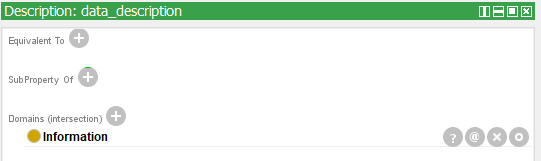
\includegraphics[width=10cm]{../../Images/04_Contribution/04_data_description.png}
  \caption{If $Information$ is the domain of the property $data\_description$, then the reasoner will infer individuals that have a $data\_description$ as $Information$.}
  \label{fig:04_data_description}
\end{figure}

\paragraph{Inconsistency}
Code sample \ref{GODP_COMP} presents the generic ontology design pattern to create a data property. This code sample includes a range. The definition of the range limits the data range that the data property accepts, for example, a $xsd:string$ accepts strings or $xsd:int$ accepts integers. The ontology is inconsistent when the data property stores a value that is outside of the defined range.

\paragraph{Generic ontology design pattern}
Code sample \ref{GODP_COMP} adds a data property or an object property to an existing class. We use three parameters to instantiate the data or object property: $c$ defines the class that should host the data property, $p$ defines the data property itself, and $r$ defines the range of the data property. We use the range of the data property to restrict its content using, for example, regular expressions and use the range of the object property to infer the class of an individual. Figure \ref{fig:GODP_COMP_DP} presents the data property, and figure \ref{fig:GODP_COM_OP} presents the object property.

\begin{lstlisting}[float,language=GDOL,caption={The GDOL code for adding a required data property to an existing class using two parameters. We use $c$, $i$, and $r$ as parameters to instantiate the data or object property.},label={GODP_COMP}][H]
pattern Completeness_dp [Class: c; DataProperty: i; Datatype: r] =
	DataProperty: i Domain: c Range: r
pattern Completeness_op [Class: c; ObjectProperty: i; Datatype: r] =
	ObjectProperty: i Domain: c Range: r
\end{lstlisting}

\begin{figure}[H]
\centering
  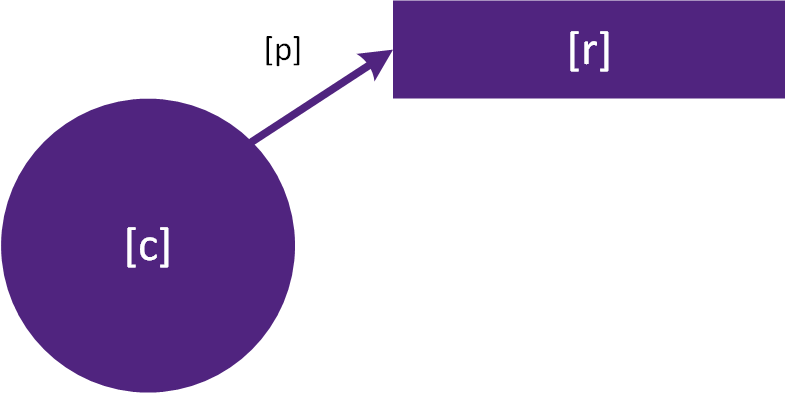
\includegraphics[width=5cm]{../../Images/04_Contribution/Completeness_DP.png}
  \caption{The completeness of a class using a data property. Code sample \ref{GODP_COMP} presents the GDOL code for adding a data property to an existing class. Code sample \ref{GODP_COMP} presents the GDOL code that instantiates this ontology.}
  \label{fig:GODP_COMP_DP}
\end{figure} 

\begin{figure}[H]
\centering
  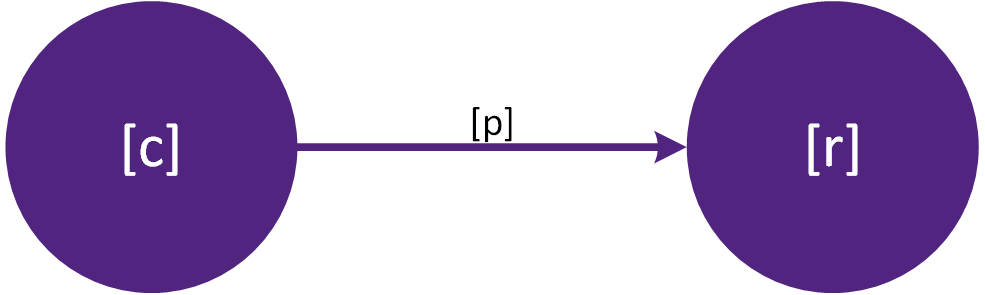
\includegraphics[width=6cm]{../../Images/04_Contribution/Completeness_OP.png}
  \caption{The completeness of a class using an object property. Code sample \ref{GODP_COMP} presents the GDOL code for adding an object property to an existing class. Code sample \ref{GODP_COMP} presents the GDOL code that instantiates this ontology.}
  \label{fig:GODP_COM_OP}
\end{figure} 

\paragraph{Constraints}
The SHACL shape in code sample \ref{SHACL_COM_DP} detects when an individual classified as $c$ does not host the defined data or object property $p$. Each individual classified as $c$ should have at least one path (object or data property) $p$. The SHACL shape monitors the existence of the data or object property using the cardinality constraint $minCount$. $c$ and $p$ set the context of the constraints.

\begin{lstlisting}[float,language=SHACL,caption={The SHACL code that validates if the individuals classified as $c$ host the property $p$. We use the cardinality constraint $sh:minCount$ for this detection: each individual classified as $c$ should have at least one path (object or data property) $p$.},label={SHACL_COM_DP}][H]
[c]Shape a sh:NodeShape;
	sh:targetClass [c]; 
	sh:property [
		sh:path [p]; 
		sh:severity sh:Violation; 
		sh:minCount 1; 
		sh:message "Completeness: add [c] to [p]."; ]
\end{lstlisting}